\documentclass[a4paper,11pt,fleqn]{article}%fleqn pour aligner les equations à gauche
\usepackage{/home/rweye/Nextcloud/Documents/Overleaf/Styles/Exercice}

\newcommand{\chnum}{Chapitre 14}
\newcommand{\chtitle}{Émission et perception d'un son}
\newcommand{\dtype}{Exercices}


\begin{document}
\maketitle

\begin{multicols}{2}
\section{Lecture de période}
Déterminer, avec précision, la période du signal sonore modélisé ci-dessous. Calculer sa fréquence.
\begin{center}
	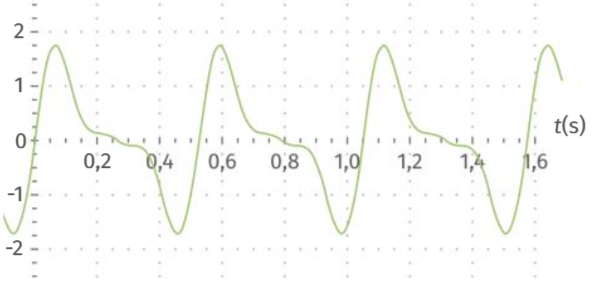
\includegraphics[scale=.5]{Ressources/2GT_C3_Exercices_Fig1.png}
\end{center}

\section{Distance parcourue}
Le son d'une balle de tennis frappée se déplace à la vitesse $v$ = \SI{340}{\meter\per\second}.\\
A quelle distance de notre oreille a-t-elle été frappée si le son nous arrive $\Delta t$ = \SI{0.12}{s} après le choc ?

\section{Le pétard}
Le 14 juillet à la nuit tombante, on observe depuis un ponton sur le lac un pétard qui explose sur la rive opposée. La carte de randonnée mentionne que les deux endroits sont distants de $d_{lac}$ = \SI{480}{m}. On mesure la durée $\Delta t$ = \SI{1,4}{s} entre la lueur de l'explosion et la perception du con de l'éclatement.
\begin{enumerate}
	\item Rappeler la relation qui lie la célérité de la lumière $v_{lum}$, sa durée de propagation $\Delta t$ et la distance $d_{lac}$.
	\item En déduire la durée $\Delta t$ mise par la lumière pour traverser le lac jusqu'à notre \oe il.
	\item Justifier que l'on peut considérer avoir vu l'explosion instantanément.
	\item Que représente alors aussi $\Delta t$ ?
	\item Pourquoi peut-on écrire $v_{son}=\dfrac{d_{lac}}{\Delta t}$ ?
	\item Calculer $v_{son}$. Le résultat est-il cohérent avec la valeur du cours ?
\end{enumerate}

\section{Le poteau, la masse et le champ}
Le père de Léo plante des poteaux au bout de son champ pour préparer un enclos. Léo, à l'autre extrémité du terrain, constate qu'il entend le choc de la masse sur le poteau alors que la masse est déjà remontée.\\
Il mesure $\Delta t$ = \SI{0.5}{s} entre l'instant du choc et l'instant où il perçoit le son.
\begin{enumerate}
	\item Pourquoi observe-t-il un décalage entre le son perçu et l'image visible du choc ?
	\item Exprimer $v_{son}$ en fonction de $\Delta t$ et $L$, la longueur du terrain.
	\item Calculer $L$.
\end{enumerate}


\section{Où est tombée la foudre ?}
On voit un éclair lors d'un orage, et le tonnerre se fait entendre \SI{2.3}{s} après. On désire estimer à quelle distance se trouve l'impact de la foudre.
\begin{enumerate}
	\item Donner les étapes du raisonnement en justifiant les approximations faites.
	\item Calculer la distance de l'impact.
\end{enumerate}

\noindent \colorbox{red!10}{
	\begin{minipage}{.48\textwidth}
		\textbf{Données : }
		\begin{itemize}
			\item \textbf{Célérité de la lumière dans l'air :} \\ $c$ = \SI{3.00E8}{\meter\per\second}
			\item \textbf{Célérité du son dans l'air à \SI{20}{\celsius} :}\\ $v_{son}$ = \SI{340}{\meter\per\second}
		\end{itemize}
	\end{minipage}}

\section{Accordage d'une guitare}
Maëlle veut accorder la guitare de manière à ce qu'elle joue des sons de même hauteur que les autres instruments de son groupe. Elle joue un La3 qui devrait correspondre à une fréquence de \SI{440}{\hertz}. L'enregistrement du son donne la courbe suivante :
\begin{center}
	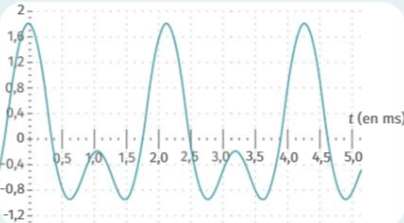
\includegraphics[scale=.5]{Ressources/2GT_C3_Exercices_Fig2.png}
\end{center}

\begin{enumerate}
	\item La guitare est-elle bien accordée ?
	\item Tendre la corde donne un son plus aigu. Ici, doit-on la tendre ou la détendre ? Justifier.
	\item Quelle est l'utilité de la caisse de résonance en bois de la guitare ?
	\item Quel(s) paramètre(s) du son perçu est/dont modifié(s) par la caisse de résonance : don intensité, sa fréquence, sa période ? Justifier.
	\item Dans le cas d'une \emph{silent guitar}, par quoi la caisse de résonance est-elle remplacée ? Quel est son intérêt ?
\end{enumerate}
\end{multicols}
\end{document}